\documentclass{beamer}

\usepackage{amsmath, amssymb}
%\usepackage[utf8]{inputenc}
\usepackage{animate}
\usepackage{zxjatype}
\usepackage[ipa]{zxjafont}
\usepackage{mymacro}
\usepackage{booktabs}
\usepackage{tikz}
\usetikzlibrary{arrows.meta, positioning, calc}

\usefonttheme{professionalfonts}
\setbeamertemplate{navigation symbols}{}

% --- page number ---
\setbeamertemplate{footline}{%
	\raisebox{10pt}{\makebox[\paperwidth]{\hfill\makebox[7em]{\normalsize\texttt{\insertframenumber/\inserttotalframenumber}}}}%
}

% Presenter's note
% \setbeameroption{show notes on second screen}

\title{Motion-enabled tomography via Gaussian mixture models}
\author{Daniel Burrows, Can Evren Yarman, Ozan \"Oktem}
% \date{\today}
\date{20th March 2026}

\begin{document}

    %%%%%%%%%%%%%%%%%%%%%%%%%%%%%%%%%%%%%%%%%%%%%%%%%%%%%%%%%%%%%%%%%%%%%%%%%%%%%%%%%%%%%%%%%%%%%%%%%%%%%%%%%%%%
    % SLIDE 1: Title
    %%%%%%%%%%%%%%%%%%%%%%%%%%%%%%%%%%%%%%%%%%%%%%%%%%%%%%%%%%%%%%%%%%%%%%%%%%%%%%%%%%%%%%%%%%%%%%%%%%%%%%%%%%%%
    \begin{frame}[plain]
        \maketitle
    \end{frame}

    %%%%%%%%%%%%%%%%%%%%%%%%%%%%%%%%%%%%%%%%%%%%%%%%%%%%%%%%%%%%%%%%%%%%%%%%%%%%%%%%%%%%%%%%%%%%%%%%%%%%%%%%%%%%
    % SLIDE 2: Motivation
    %%%%%%%%%%%%%%%%%%%%%%%%%%%%%%%%%%%%%%%%%%%%%%%%%%%%%%%%%%%%%%%%%%%%%%%%%%%%%%%%%%%%%%%%%%%%%%%%%%%%%%%%%%%%
    \begin{frame}{Motivation}

        \textbf{Standard CT:} scanner rotates around a stationary object. \\[0.8em]

        \pause
        \textbf{Goal:} scan objects \emph{as they move} through a fixed beam.
        \begin{itemize}
            \item No moving parts \quad$\Rightarrow$\quad high throughput
            \item Natural tumbling \quad$\Rightarrow$\quad more angular views
        \end{itemize}

        \pause
        \vspace{0.6em}
        \textbf{Application:} rapid automated imaging of rock fragments from geological drilling.

        \note{CT is widely understood. The key idea: remove the stationary requirement. Motion actually helps by providing more views. Geological drilling application motivates the geometry.}
    \end{frame}

    %%%%%%%%%%%%%%%%%%%%%%%%%%%%%%%%%%%%%%%%%%%%%%%%%%%%%%%%%%%%%%%%%%%%%%%%%%%%%%%%%%%%%%%%%%%%%%%%%%%%%%%%%%%%
    % SLIDE 3: The challenge
    %%%%%%%%%%%%%%%%%%%%%%%%%%%%%%%%%%%%%%%%%%%%%%%%%%%%%%%%%%%%%%%%%%%%%%%%%%%%%%%%%%%%%%%%%%%%%%%%%%%%%%%%%%%%
    \begin{frame}{The challenge: CT of objects in motion}
        \begin{columns}[T]
            \begin{column}{0.55\textwidth}
                \textbf{Setup:} Fixed source $\mathbf{s}$ and detector --- objects rotate as they move through the gantry.

                \vspace{0.5em}
                \begin{itemize}
                    \item Single source $\Rightarrow$ limited-angle tomography
                    \item Object motion $\Rightarrow$ transforms it to finite-angle tomography
                    \item Additional complexity: must recover \emph{dynamics} jointly with structure
                \end{itemize}

                \vspace{0.5em}
                \textbf{Approach:} Model each particle as a Gaussian.
                \begin{itemize}
                    \item GMMs approximate general objects to arbitrary accuracy
                    \item Closed under the ray transform
                \end{itemize}
            \end{column}
            \begin{column}{0.42\textwidth}
                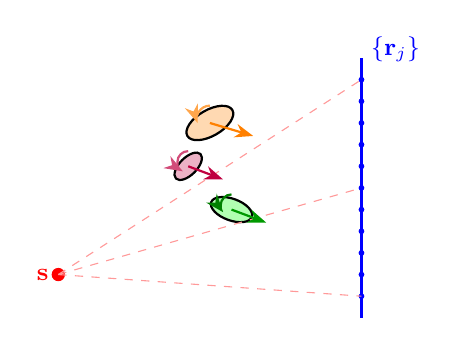
\begin{tikzpicture}[scale=0.55, every node/.style={font=\small}]
                    % Source
                    \filldraw[red] (-3, -2) circle (4pt) node[left] {$\mathbf{s}$};

                    % Receiver array
                    \draw[thick, blue] (4, -3) -- (4, 3);
                    \foreach \y in {-2.5, -2, ..., 2.5} {
                        \filldraw[blue] (4, \y) circle (1.5pt);
                    }
                    \node[blue, right] at (4, 3.2) {$\{\mathbf{r}_j\}$};

                    % Objects (ellipses)
                    \draw[thick, fill=orange!30, rotate around={30:(0.5, 1.5)}] (0.5, 1.5) ellipse (0.6 and 0.3);
                    \draw[thick, fill=green!30, rotate around={-20:(1.0, -0.5)}] (1.0, -0.5) ellipse (0.5 and 0.25);
                    \draw[thick, fill=purple!30, rotate around={45:(0.0, 0.5)}] (0.0, 0.5) ellipse (0.4 and 0.2);

                    % Fan beam rays
                    \draw[red!40, dashed] (-3, -2) -- (4, 2.5);
                    \draw[red!40, dashed] (-3, -2) -- (4, 0);
                    \draw[red!40, dashed] (-3, -2) -- (4, -2.5);

                    % Trajectory arrows
                    \draw[-{Stealth}, thick, orange] (0.5, 1.5) -- (1.5, 1.2);
                    \draw[-{Stealth}, thick, green!60!black] (1.0, -0.5) -- (1.8, -0.8);
                    \draw[-{Stealth}, thick, purple] (0.0, 0.5) -- (0.8, 0.2);

                    % Rotation arcs
                    \draw[-{Stealth}, thick, orange!70] (0.5, 1.9) arc (90:200:0.3);
                    \draw[-{Stealth}, thick, green!50!black] (1.0, -0.15) arc (90:220:0.25);
                    \draw[-{Stealth}, thick, purple!70] (0.0, 0.85) arc (90:240:0.25);
                \end{tikzpicture}
            \end{column}
        \end{columns}

        \note{The key insight is that motion, which is normally a nuisance in CT, actually provides additional angular information when the objects rotate. This converts limited-angle into finite-angle tomography. We model particles as Gaussians because GMMs are closed under the ray transform.}
    \end{frame}

    %%%%%%%%%%%%%%%%%%%%%%%%%%%%%%%%%%%%%%%%%%%%%%%%%%%%%%%%%%%%%%%%%%%%%%%%%%%%%%%%%%%%%%%%%%%%%%%%%%%%%%%%%%%%
    % SLIDE 4: The mathematical setting
    %%%%%%%%%%%%%%%%%%%%%%%%%%%%%%%%%%%%%%%%%%%%%%%%%%%%%%%%%%%%%%%%%%%%%%%%%%%%%%%%%%%%%%%%%%%%%%%%%%%%%%%%%%%%
    \begin{frame}{Mathematical setting}
        \textbf{Object model:} $N$ rigid particles with independent motions,
        $$
            f(\mathbf{x}, t) = \sum_{n=1}^{N} \bigl(M_n(t).U_n^{-1}.\rho_0\bigr)(\mathbf{x}), \qquad \rho_0(\mathbf{x}) := e^{-\mathbf{x}^\top \mathbf{x}}
        $$
        where $M_n(t) = \bigl(R_{\Omega_n}(t),\, \tau_n(t)\bigr) \in \mathrm{SE}(d)$ encodes rigid body motion.

        \vspace{0.5em}
        \pause
        \textbf{Particle morphology:} $\rho_n(\mathbf{x}) = \alpha_n \rho_0(U_n \mathbf{x})$, \quad $U_n$ upper triangular, \, $\alpha_n > 0$.

        \vspace{0.5em}
        \textbf{Projectile motion:}\quad $C[\eta_n](t) = \boldsymbol{\mu} + t\mathbf{v}_n + \tfrac{t^2}{2}\mathbf{a}$

        \vspace{0.3em}
        \textbf{Rotation:}\quad $R_{\Omega_n}(t) = \prod_{k=1}^{d_R} R_k(t\theta_{n,k})$, \quad $d_R = \binom{d}{2}$

        \vspace{0.5em}
        \textbf{Parameter vector per particle:}
        $$
            \gamma_n = \bigl((\alpha_n, U_n),\, \eta_n\bigr) \in (\mathbb{R} \times \mathbb{R}^{d_U}) \times (\mathbb{R}^d \times \mathbb{R}^{d_R} \times \mathbb{R}^d \times \mathbb{R}^d)
        $$

        \note{Present the generative model. Each particle has attenuation $\alpha_n$, shape $U_n$, and motion parameters $\eta_n = (\mu, \Theta_n, v_n, a)$. The morphology component generates particles in the GL(d) orbit of $\rho_0$.}
    \end{frame}

    %%%%%%%%%%%%%%%%%%%%%%%%%%%%%%%%%%%%%%%%%%%%%%%%%%%%%%%%%%%%%%%%%%%%%%%%%%%%%%%%%%%%%%%%%%%%%%%%%%%%%%%%%%%%
    % SLIDE 5: Demo --- show the notebook animation
    %%%%%%%%%%%%%%%%%%%%%%%%%%%%%%%%%%%%%%%%%%%%%%%%%%%%%%%%%%%%%%%%%%%%%%%%%%%%%%%%%%%%%%%%%%%%%%%%%%%%%%%%%%%%
    \begin{frame}{Demo: Simulated GMM in motion}
        \centering
        {\Large \textit{[Live demo --- notebook]}}

        \vspace{1em}
        \texttt{gmm-ct\_notebook.ipynb} --- Cells 4 \& 8

        \vspace{1em}
        \begin{itemize}
            \item $N$ anisotropic Gaussians with independent trajectories and rotations
            \item Fan-beam X-ray projections evolving in time
            \item Sinogram data $g[\mathbf{m}] \approx F[\Gamma](\mathbf{s}, \mathbf{r}_{m_r}, t_{m_t})$ recorded at each time step
        \end{itemize}

        \note{Switch to the notebook and run the GMM animation. Show how the particles move through the field of view, rotating and translating, producing time-varying projections.}
    \end{frame}

    %%%%%%%%%%%%%%%%%%%%%%%%%%%%%%%%%%%%%%%%%%%%%%%%%%%%%%%%%%%%%%%%%%%%%%%%%%%%%%%%%%%%%%%%%%%%%%%%%%%%%%%%%%%%
    % SLIDE 6: Forward model --- the ray transform
    %%%%%%%%%%%%%%%%%%%%%%%%%%%%%%%%%%%%%%%%%%%%%%%%%%%%%%%%%%%%%%%%%%%%%%%%%%%%%%%%%%%%%%%%%%%%%%%%%%%%%%%%%%%%
    \begin{frame}{Forward model: Closure under the ray transform}
        \textbf{Ray transform} (Definition 5.1):
        $$
            \mathcal{X}\bigl(f(\cdot, t)\bigr)[\mathbf{s}, \mathbf{r}] := \int_{\mathbb{R}} f\bigl(\mathbf{s} + \xi\,\widehat{\mathbf{r} - \mathbf{s}},\, t\bigr)\,d\xi
        $$

        \pause
        \vspace{0.3em}
        \textbf{Proposition 5.2.} For $A = (U^{-1}, \boldsymbol{\mu}) \in \mathrm{Aff}(d)$, the ray transform of $A.\rho_0$ is:
        $$
            \mathcal{X}(A.\rho_0)[\mathbf{s}, \mathbf{r}]
            = \frac{\sqrt{\pi}}{\|U(\mathbf{r} - \mathbf{s})\|}
            \exp\!\left(
            \frac{
              \bigl\langle U(\mathbf{r} - \mathbf{s}),\; U(\mathbf{s} - \boldsymbol{\mu})\bigr\rangle^2
            }{
              \|U(\mathbf{r} - \mathbf{s})\|^2
            }
            - \|U(\mathbf{s} - \boldsymbol{\mu})\|^2\right)
        $$

        \vspace{0.3em}
        \textbf{Forward operator:}
        $\displaystyle
            F[\Gamma](\mathbf{s}, \mathbf{r}, t) = \sum_{n=1}^{N} \alpha_n\, \mathcal{X}\bigl(A[U_n, \eta_n](t).\rho_0\bigr)[\mathbf{s}, \mathbf{r}]
        $

        \vspace{0.3em}
        \begin{itemize}
            \item Exact --- no numerical quadrature
            \item Fully differentiable $\Rightarrow$ gradient-based optimisation via PyTorch
        \end{itemize}

        \note{The key result: the ray transform of a Gaussian has a closed form. This is the engine of the whole method. It means we can evaluate and differentiate the forward model exactly.}
    \end{frame}

    %%%%%%%%%%%%%%%%%%%%%%%%%%%%%%%%%%%%%%%%%%%%%%%%%%%%%%%%%%%%%%%%%%%%%%%%%%%%%%%%%%%%%%%%%%%%%%%%%%%%%%%%%%%%
    % SLIDE 7: The inverse problem and decoupling
    %%%%%%%%%%%%%%%%%%%%%%%%%%%%%%%%%%%%%%%%%%%%%%%%%%%%%%%%%%%%%%%%%%%%%%%%%%%%%%%%%%%%%%%%%%%%%%%%%%%%%%%%%%%%
    \begin{frame}{The inverse problem}
        \textbf{Recover} $\Gamma = (\gamma_1, \ldots, \gamma_N)$ from data $g[\mathbf{m}] \approx F[\Gamma](\mathbf{s}, \mathbf{r}_{m_r}, t_{m_t})$ \textbf{(Definition 6.1)}:
        $$
            \Gamma^* \in \arg\min_{\Gamma}\, L\bigl(\{g_m\},\; \{F[\Gamma](s_m, r_m, t_m)\}\bigr)
        $$

        \pause
        \vspace{0.3em}
        \textbf{Key insight:} Split $\Gamma = [\Gamma_D,\, \Gamma_S]$ into dynamic and static parts and decouple:
        \begin{align*}
            \Gamma_D^i &\in \arg\min_{\Gamma_D}\, L_D\bigl(\{g_m\},\; F[\Gamma_D, \Gamma_S^{i-1}]\bigr)
            && \text{(Trajectories)} \\[4pt]
            \Gamma_S^i &\in \arg\min_{\Gamma_S}\, L_S\bigl(\{g_m\},\; F[\Gamma_D^i, \Gamma_S]\bigr)
            && \text{(Morphology)}
        \end{align*}

        \vspace{0.3em}
        If $L_D$ depends only on \textbf{modes} of the projections, then by \textbf{Proposition 6.2} the trajectory estimate $\Gamma_D^*$ is \emph{independent of morphology} $\Gamma_S$. \\[3pt]
        $\Rightarrow$ Alternating scheme becomes \textbf{sequential}: first trajectories, then morphology.

        \note{The non-convexity of the full problem is addressed by decoupling. Proposition 6.2 shows that the modes of the ray transform of an isotropic Gaussian are independent of $U$ --- they only depend on the source and the trajectory. This is what makes the sequential approach work.}
    \end{frame}

    %%%%%%%%%%%%%%%%%%%%%%%%%%%%%%%%%%%%%%%%%%%%%%%%%%%%%%%%%%%%%%%%%%%%%%%%%%%%%%%%%%%%%%%%%%%%%%%%%%%%%%%%%%%%
    % SLIDE 8: Mode-based trajectory recovery
    %%%%%%%%%%%%%%%%%%%%%%%%%%%%%%%%%%%%%%%%%%%%%%%%%%%%%%%%%%%%%%%%%%%%%%%%%%%%%%%%%%%%%%%%%%%%%%%%%%%%%%%%%%%%
    \begin{frame}{Trajectory recovery: Mode-based approach}
        \textbf{Proposition 6.2.} The mode of $\mathbf{r} \mapsto \mathcal{X}(A.\rho_0)[\mathbf{s}, \mathbf{r}]$ is collinear with $\mathbf{s}$ and $\boldsymbol{\mu}$, \emph{independently of} $U$.

        \vspace{0.3em}
        \pause
        \textbf{Data modes} $M[g](t)$: local maxima of $g[\mathbf{m}]$ w.r.t.\ receiver locations.

        \textbf{Projected trajectories} $\mathcal{C}_{\mathcal{X}}[\eta_n](t)$: receivers closest to the projection of $C[\eta_n](t)$ through $\mathbf{s}$.

        \vspace{0.3em}
        \textbf{Trajectory loss} --- approximate Hausdorff matching:
        $$
            L_D = \sum_{m_t=1}^{M_t} \sum_{n=1}^{N} d_H\bigl(M[g](t_{m_t}),\; \mathcal{C}_{\mathcal{X}}[\eta_n](t_{m_t})\bigr)
        $$

        \vspace{0.3em}
        \pause

        In practice, use the \textbf{Hungarian algorithm} to compute optimal assignments between data modes and predicted modes at each $t_k$.

        \vspace{0.3em}
        Optimised via \textbf{multi-start L-BFGS} ($N_{\mathrm{traj}}$ random initialisations).

        \note{The mode-based loss avoids the vanishing gradient problem of the full $L^2$ loss. The Hungarian algorithm provides optimal bipartite matching at each time step. Multi-start L-BFGS explores the landscape.}
    \end{frame}

    %%%%%%%%%%%%%%%%%%%%%%%%%%%%%%%%%%%%%%%%%%%%%%%%%%%%%%%%%%%%%%%%%%%%%%%%%%%%%%%%%%%%%%%%%%%%%%%%%%%%%%%%%%%%
    % SLIDE 9: Demo --- trajectory recovery and full reconstruction
    %%%%%%%%%%%%%%%%%%%%%%%%%%%%%%%%%%%%%%%%%%%%%%%%%%%%%%%%%%%%%%%%%%%%%%%%%%%%%%%%%%%%%%%%%%%%%%%%%%%%%%%%%%%%
    \begin{frame}{Demo: Trajectory and morphology recovery}
        \centering
        {\Large \textit{[Live demo --- notebook]}}

        \vspace{1em}
        \begin{enumerate}
            \item Na\"ive $L^2$ trajectory optimisation fails (Cell 15) \\
                  \small{\texttt{direct\_traj\_est.gif}}\normalsize
            \vspace{0.3em}
            \item Peak detection and mode visualisation (Cell 19)
            \vspace{0.3em}
            \item Mode-based trajectory recovery with Hungarian assignment (Cells 24--28) \\
                  \small{\texttt{Hungarian\_traj\_est.gif}}\normalsize
            \vspace{0.3em}
            \item Full joint reconstruction, Stages 2--4 (Cell 30) \\
                  \small{\texttt{temporal\_gmm\_comparison\_n\_inits=\{n\}.gif}}\normalsize
        \end{enumerate}

        \note{Walk through the notebook demos. First show the failure of na\"ive L2, then the mode detection, then the successful trajectory recovery, and finally the full morphology reconstruction. This is the core demo of the talk.}
    \end{frame}

    %%%%%%%%%%%%%%%%%%%%%%%%%%%%%%%%%%%%%%%%%%%%%%%%%%%%%%%%%%%%%%%%%%%%%%%%%%%%%%%%%%%%%%%%%%%%%%%%%%%%%%%%%%%%
    % SLIDE 10: Numerical results --- N=5 and N=10
    %%%%%%%%%%%%%%%%%%%%%%%%%%%%%%%%%%%%%%%%%%%%%%%%%%%%%%%%%%%%%%%%%%%%%%%%%%%%%%%%%%%%%%%%%%%%%%%%%%%%%%%%%%%%
    \begin{frame}{Results: $N = 5$ and $N = 10$}
        \begin{columns}[T]
            \begin{column}{0.48\textwidth}
                \textbf{$N = 5$} --- strong recovery:
                \vspace{0.2em}

                \small
                \begin{tabular}{@{}lcc@{}}
                    \toprule
                     & Init.\ err & Final err \\
                    \midrule
                    $\{\alpha_n\}$ & $5.52\!\times\!10^{-1}$ & $9.83\!\times\!10^{-3}$ \\
                    $\{v_n\}$      & $1.13\!\times\!10^{0\phantom{-}}$  & $5.01\!\times\!10^{-3}$ \\
                    $\{U_n\}$      & $4.70\!\times\!10^{-1}$ & $1.88\!\times\!10^{-2}$ \\
                    $\{\Theta_n\}$ & $1.00\!\times\!10^{0\phantom{-}}$  & $3.91\!\times\!10^{-4}$ \\
                    Proj.          & $9.43\!\times\!10^{-1}$ & $5.05\!\times\!10^{-2}$ \\
                    \bottomrule
                \end{tabular}
                \normalsize
            \end{column}
            \begin{column}{0.48\textwidth}
                \textbf{$N = 10$} --- saturated data:
                \vspace{0.2em}

                \small
                \begin{tabular}{@{}lcc@{}}
                    \toprule
                     & Init.\ err & Final err \\
                    \midrule
                    $\{\alpha_n\}$ & $7.06\!\times\!10^{-1}$ & $3.85\!\times\!10^{-1}$ \\
                    $\{v_n\}$      & $1.06\!\times\!10^{0\phantom{-}}$  & $1.50\!\times\!10^{-1}$ \\
                    $\{U_n\}$      & $5.68\!\times\!10^{-1}$ & $3.46\!\times\!10^{2\phantom{-}}$ \\
                    $\{\Theta_n\}$ & $1.00\!\times\!10^{0\phantom{-}}$  & $7.91\!\times\!10^{-2}$ \\
                    Proj.          & $9.72\!\times\!10^{-1}$ & $8.85\!\times\!10^{-2}$ \\
                    \bottomrule
                \end{tabular}
                \normalsize
            \end{column}
        \end{columns}

        \vspace{0.5em}
        \begin{itemize}
            \item $N = 5$: excellent recovery in both parameter and projection space
            \item $N = 10$: projection fit remains strong; \emph{parameter} accuracy limited by identifiability (obscured particles)
            \item Poor recovery of one particle (fully obscured by another) is \emph{localised} --- does not affect other estimates
        \end{itemize}

        \note{Walk through Tables 1 and 2 from the paper. The $N=10$ case has one particle completely obscured by another ($\rho_4$ behind $\rho_6$), yet the projection fit remains good and recovery of the remaining particles is strong. The skewness error is dominated by the single unobservable particle.}
    \end{frame}

    %%%%%%%%%%%%%%%%%%%%%%%%%%%%%%%%%%%%%%%%%%%%%%%%%%%%%%%%%%%%%%%%%%%%%%%%%%%%%%%%%%%%%%%%%%%%%%%%%%%%%%%%%%%%
    % SLIDE 11: Stability analysis
    %%%%%%%%%%%%%%%%%%%%%%%%%%%%%%%%%%%%%%%%%%%%%%%%%%%%%%%%%%%%%%%%%%%%%%%%%%%%%%%%%%%%%%%%%%%%%%%%%%%%%%%%%%%%
    \begin{frame}{Stability analysis: $N_{\mathrm{sim}} = 50$ trials per $N$}
        % Accuracy metric: Accuracy(theta) = (1 - ||theta - theta_true|| / ||theta_true||) * 100%
        \begin{columns}[T]
            \begin{column}{0.48\textwidth}
                \centering
                \textbf{Parameter accuracy}

                \vspace{0.3em}
                \small
                \begin{tabular}{@{}cccc@{}}
                    \toprule
                    $N$ & Mean & Std & Valid \\
                    \midrule
                    1  & 98.9\% & 1.6\% & 49/50 \\
                    3  & 91.1\% & 14.0\% & 50/50 \\
                    5  & 84.1\% & 13.8\% & 48/50 \\
                    7  & 68.5\% & 13.2\% & 50/50 \\
                    10 & 59.8\% & 12.0\% & 48/50 \\
                    \bottomrule
                \end{tabular}
                \normalsize
            \end{column}
            \begin{column}{0.48\textwidth}
                \centering
                \textbf{Projection accuracy}

                \vspace{0.3em}
                \small
                \begin{tabular}{@{}ccc@{}}
                    \toprule
                    $N$ & Mean & Std \\
                    \midrule
                    1  & 95.7\% & 2.6\% \\
                    3  & 93.5\% & 3.6\% \\
                    5  & 87.9\% & 10.7\% \\
                    7  & 83.3\% & 9.3\% \\
                    10 & 75.7\% & 13.1\% \\
                    \bottomrule
                \end{tabular}
                \normalsize
            \end{column}
        \end{columns}

        \vspace{0.5em}
        \begin{itemize}
            \item Decrease in parameter accuracy is mostly due to \emph{obscured particles} --- local accuracy remains high for observable particles
            \item Only 9 of 500 total runs (1.8\%) failed
            \item Projection space accuracy degrades more gracefully
        \end{itemize}

        \note{From Figure 5 and Table 4 in the paper. The key observation is that the method recovers particles that it can observe, and the failure to recover obscured particles remains localised. The gap between local and global accuracy widens with $N$, consistent with an increasing proportion of obscured particles.}
    \end{frame}

    %%%%%%%%%%%%%%%%%%%%%%%%%%%%%%%%%%%%%%%%%%%%%%%%%%%%%%%%%%%%%%%%%%%%%%%%%%%%%%%%%%%%%%%%%%%%%%%%%%%%%%%%%%%%
    % SLIDE 12: Conclusions and future work
    %%%%%%%%%%%%%%%%%%%%%%%%%%%%%%%%%%%%%%%%%%%%%%%%%%%%%%%%%%%%%%%%%%%%%%%%%%%%%%%%%%%%%%%%%%%%%%%%%%%%%%%%%%%%
    \begin{frame}{Conclusions and future work}
        \textbf{Summary:}
        \begin{itemize}
            \item GMMs are closed under the ray transform $\Rightarrow$ exact, differentiable forward model
            \item Mode-based trajectory recovery decouples dynamics from morphology
            \item Multi-stage optimisation achieves accurate reconstruction in challenging scenarios
            \item Error from unobservable particles remains \emph{localised}
        \end{itemize}

        \vspace{0.5em}
        \pause
        \textbf{Future work:}
        \begin{itemize}
            \item Extension to $d = 3$ (trajectory recovery requires a non-explicit map in higher dimensions)
            \item Robustness to noise in the sinogram data
            \item Clumped Gaussians for complex, asymmetric structures
            \item Unknown initial locations and bidirectional rotations
            \item Regularisation to penalise unrealistic solutions
            \item Optimal experimental design: minimal receiver configurations
        \end{itemize}

        \note{Emphasise that the framework is valid in arbitrary dimension, but the current 2D trajectory recovery exploits an explicit map. In 3D, this needs adaptation. Noise handling and more complex particle models are natural next steps. The optimal experimental design problem (cited in the paper) is left for future work.}
    \end{frame}

    %%%%%%%%%%%%%%%%%%%%%%%%%%%%%%%%%%%%%%%%%%%%%%%%%%%%%%%%%%%%%%%%%%%%%%%%%%%%%%%%%%%%%%%%%%%%%%%%%%%%%%%%%%%%
    % SLIDE 13: Thank you
    %%%%%%%%%%%%%%%%%%%%%%%%%%%%%%%%%%%%%%%%%%%%%%%%%%%%%%%%%%%%%%%%%%%%%%%%%%%%%%%%%%%%%%%%%%%%%%%%%%%%%%%%%%%%
    \begin{frame}[plain]
        \centering
        \vspace{2cm}
        {\Huge Thank you}

        \vspace{1.5cm}
        {\large Questions?}

        \vspace{1.5cm}
        {\small Code: \texttt{https://github.com/dwb26/GaussCT}}
    \end{frame}

\end{document}
